%%%%%%%%%%%%%%%%%%%%%%%%%%%%%%%%%%%%%%%%%
% Masters/Doctoral Thesis 
% LaTeX Template
% Version 2.5 (27/8/17)
%
% This template was downloaded from:
% http://www.LaTeXTemplates.com
%
% Version 2.x major modifications by:
% Vel (vel@latextemplates.com)
%
% This template is based on a template by:
% Steve Gunn (http://users.ecs.soton.ac.uk/srg/softwaretools/document/templates/)
% Sunil Patel (http://www.sunilpatel.co.uk/thesis-template/)
%
% Template license:
% CC BY-NC-SA 3.0 (http://creativecommons.org/licenses/by-nc-sa/3.0/)
%
%%%%%%%%%%%%%%%%%%%%%%%%%%%%%%%%%%%%%%%%%

%----------------------------------------------------------------------------------------
%	PACKAGES AND OTHER DOCUMENT CONFIGURATIONS
%----------------------------------------------------------------------------------------

\documentclass[
11pt, % The default document font size, options: 10pt, 11pt, 12pt
oneside, % Two side (alternating margins) for binding by default, uncomment to switch to one side
spanish, % ngerman for German
singlespacing, % Single line spacing, alternatives: onehalfspacing or doublespacing
%draft, % Uncomment to enable draft mode (no pictures, no links, overfull hboxes indicated)
%nolistspacing, % If the document is onehalfspacing or doublespacing, uncomment this to set spacing in lists to single
%liststotoc, % Uncomment to add the list of figures/tables/etc to the table of contents
%toctotoc, % Uncomment to add the main table of contents to the table of contents
% parskip, % Uncomment to add space between paragraphs
%nohyperref, % Uncomment to not load the hyperref package
headsepline, % Uncomment to get a line under the header
%chapterinoneline, % Uncomment to place the chapter title next to the number on one line
%consistentlayout, % Uncomment to change the layout of the declaration, abstract and acknowledgements pages to match the default layout
]{MastersDoctoralThesis} % The class file specifying the document structure

\usepackage[utf8]{inputenc} % Required for inputting international characters
\usepackage[T1]{fontenc} % Output font encoding for international characters

\usepackage{mathpazo} % Use the Palatino font by default
\usepackage{lipsum}
\usepackage[acronym, toc]{glossaries}

\usepackage[backend=bibtex,style=numeric,natbib=true]{biblatex} % Use the bibtex backend with the authoryear citation style (which resembles APA)

\addbibresource{references.bib} % The filename of the bibliography

\usepackage[autostyle=true]{csquotes} % Required to generate language-dependent quotes in the bibliography

% \usepackage[letterpaper,landscape,margin=3cm]{geometry}
\usepackage{tikz}
\usetikzlibrary{calc}

% GanttHeader setups some parameters for the rest of the diagram
% #1 Width of the diagram
% #2 Width of the space reserved for task numbers
% #3 Width of the space reserved for task names
% #4 Number of months in the diagram
% In addition to these parameters, the layout of the diagram is influenced
% by keys defined below, such as y, which changes the vertical scale
\def\GanttHeader#1#2#3#4{%
 \pgfmathparse{(#1-#2-#3)/#4}
 \tikzset{y=7mm, task number/.style={left, font=\bfseries},
     task description/.style={text width=#3,  right, draw=none,
           font=\sffamily, xshift=#2,
           minimum height=2em},
     gantt bar/.style={draw=black, fill=red!50!black},
     help lines/.style={draw=black!30, dashed},
     x=\pgfmathresult pt
     }
  \def\totalmonths{#4}
  \node (Header) [task description] at (0,0) {\textbf{\large Actividades}};
  \begin{scope}[shift=($(Header.south east)$)]
    \foreach \x in {1,...,#4}
      \node[above] at (\x,0) {\footnotesize\x};
 \end{scope}
}

% This macro adds a task to the diagram
% #1 Number of the task
% #2 Task's name
% #3 Starting date of the task (month's number, can be non-integer)
% #4 Task's duration in months (can be non-integer)
\def\Task#1#2#3#4{%
\node[task number] at ($(Header.west) + (0, -#1)$) {#1};
\node[task description] at (0,-#1) {#2};
\begin{scope}[shift=($(Header.south east)$)]
  \draw (0,-#1) rectangle +(\totalmonths, 1);
  \foreach \x in {1,...,\totalmonths}
    \draw[help lines] (\x,-#1) -- +(0,1);
  \filldraw[gantt bar] ($(#3, -#1+0.2)$) rectangle +(#4,0.6);
\end{scope}
}

%----------------------------------------------------------------------------------------
%	MARGIN SETTINGS
%----------------------------------------------------------------------------------------

\geometry{
	paper=letterpaper, % Change to letterpaper for US letter
	inner=2.5cm, % Inner margin
	outer=3.8cm, % Outer margin
	bindingoffset=.5cm, % Binding offset
	top=1.5cm, % Top margin
	bottom=1.5cm, % Bottom margin
	%showframe, % Uncomment to show how the type block is set on the page
}

%----------------------------------------------------------------------------------------
%	THESIS INFORMATION
%----------------------------------------------------------------------------------------

\thesistitle{Advanced Natural Language Processing Techniques to Profile Cybercriminals} % Your thesis title, this is used in the title and abstract, print it elsewhere with \ttitle
\supervisor{Dr. Daniel Orlando \textsc{D\'{\i}az L\'opez}} % Your supervisor's name, this is used in the title page, print it elsewhere with \supname
\examiner{} % Your examiner's name, this is not currently used anywhere in the template, print it elsewhere with \examname
\degree{Estudiante de Ingeniería de Sistemas} % Your degree name, this is used in the title page and abstract, print it elsewhere with \degreename
\author{Alejandro \textsc{Anzola \'Avila}} % Your name, this is used in the title page and abstract, print it elsewhere with \authorname
\addresses{} % Your address, this is not currently used anywhere in the template, print it elsewhere with \addressname

\subject{Computer Science} % Your subject area, this is not currently used anywhere in the template, print it elsewhere with \subjectname
\keywords{Natural Language Processing, NLP, Cybercriminal} % Keywords for your thesis, this is not currently used anywhere in the template, print it elsewhere with \keywordnames
\university{\href{https://www.escuelaing.edu.co}{Escuela Colombiana de Ingeniería\\Julio Garavito}} % Your university's name and URL, this is used in the title page and abstract, print it elsewhere with \univname
\department{\href{https://www.escuelaing.edu.co/es/programas/pregrado/Ingenier\%C3\%ADa+de+Sistemas}{Programa de Ingeniería de Sistemas}} % Your department's name and URL, this is used in the title page and abstract, print it elsewhere with \deptname
\group{\href{ }{ }} % Your research group's name and URL, this is used in the title page, print it elsewhere with \groupname
% \faculty{\href{http://faculty.university.com}{Faculty Name}} % Your faculty's name and URL, this is used in the title page and abstract, print it elsewhere with \facname

\AtBeginDocument{
\hypersetup{pdftitle=\ttitle} % Set the PDF's title to your title
\hypersetup{pdfauthor=\authorname} % Set the PDF's author to your name
\hypersetup{pdfkeywords=\keywordnames} % Set the PDF's keywords to your keywords
}

\makeglossaries
\newcommand{\glossarydef}[4]{
    \newglossaryentry{#1}{
        text={\mbox{\textsc{#2}}},
        long={#3},
        name={#3\, \mbox{\textsc{(#2)}}},
        first={\textsl{#3}\, \mbox{\textsc{(#2)}}},
        firstplural={\textsl{\glsentrylong{#1}\glspluralsuffix}\, \mbox{(\textsc{\glsentrytext{#1}\glspluralsuffix})}},
        description={#4}
    }
}

\newcommand{\simpleglossarydef}[3]{
    \newglossaryentry{#1}{
        name={#2},
        long={#2},
        first={\textsl{#2}},
        description={#3}
    }
}

% Permite que los terminos del glosario sean en cursiva tipo 'slanted'
\let\glsentrylongnostyle\glsentrylong
\renewcommand{\glsentrylong}[1]{\textsl{\glsentrylongnostyle{#1}}}

\glossarydef{nlp}{NLP}{Natural Language Processing}{Rama de la inteligencia artificial que lidia con la interacción entre computadores y humanos usando el lenguaje natural}

\glossarydef{machinel}{ML}{Machine Learning}{Informalmente ha sido definido como ``El campo de estudio que le da a computadores la habilidad de aprender sin ser explícitamente programados'', este tiene tres tipos de algoritmos de aprendizaje: aprendizaje supervisado, aprendizaje no--supervisado, y aprendizaje por refuerzo}

\simpleglossarydef{supervisedl}{Supervised Learning}{Aprendizaje supervisado, su objetivo es aprender un mapeo de unas entradas a unas salidas definidas}

\simpleglossarydef{unsupervisedl}{Unsupervised Learning}{Aprendizaje no-supervisado, su objetivo es obtener patrones estructurados de una serie de datos no estructurados}

\simpleglossarydef{reinforcedl}{Reinforcement Learning}{Aprendizaje de refuerzo, es el aprendizaje de que acción se debe tomar de forma que se logre una señal de recompensa lo mas alto posible}

\simpleglossarydef{feedforward}{Feedforward}{Es un termino que describe típicamente un elemento o un camino dentro de un sistema de control que pasa una señal de control de una fuente externa. En la inteligencia artificial este termino no difiere en significado}

\simpleglossarydef{clustering}{Clustering}{Es la tarea de agrupar conjuntos de objetos de manera que este en grupos de mismo tipo}

\glossarydef{deepl}{DL}{Deep Learning}{Es un subcampo de Machine Learning que se usa algoritmos inspirados por la estructura y función del cerebro que son llamadas Redes Neuronales Artificiales (\'o Artificial Neural Networks en ingl\'es)}

\simpleglossarydef{dataintegration}{Data Integration}{Para acceder a múltiples y diversas fuentes de información}

\simpleglossarydef{linkanalisys}{Link Analysis}{Para visualizar asociaciones y relaciones criminales y terroristas}

\simpleglossarydef{softwareagents}{Software Agents}{Para el monitoreo, obtención, análisis y actuación sobre la información}

\simpleglossarydef{textmining}{Text Mining}{Búsqueda sobre terabytes de información en documentos, paginas web y correos electrónicos}

\simpleglossarydef{datamining}{Data Mining}{Proceso de descubrir automáticamente información útil en repositorios grandes de datos}

\glossarydef{neuralnetwork}{ANN}{Artificial Neural Network}{Para predecir la probabilidad de crímenes y nuevos ataques terroristas}

\simpleglossarydef{mlalgorithms}{Machine Learning Algorithms}{Para extraer perfiles de perpetradores y mapas gráficos de crímenes}

\glossarydef{kbs}{KBS}{Knowledge Based Systems}{Sistemas Basados en Conocimiento, su objetivo es abstraer conocimiento de un experto de un área en una representación dentro de un computador}

\glossarydef{ai}{AI}{Artificial Intelligence}{Inteligencia Artificial, área de las ciencia de la computación que se encarga de la creación de maquinas inteligentes que tienen un comportamiento que se asemeja a tener inteligencia}

\simpleglossarydef{anomalydetectionsys}{Anomaly Detection Systems}{Sistemas de Detección de Anomalías, son sistemas con el objetivo de encontrar datos atípicos dentro de un conjunto de datos, típicamente se tiene un entrenamiento previo que muestra el comportamiento típico de los datos para luego encontrar las anomalías}

\glossarydef{som}{SOM}{Self-organizing Maps}{Mapas auto-organizados, son redes neuronales especializadas para el clustering de datos semejantes según una función de distancia, da como resultado un mapa discreto uni- o bi-dimensional}

\glossarydef{svm}{SVM}{Support Vector Machine}{Maquinas de Soporte Vectorial, son modelos de aprendizaje supervisado usados para el problema de clasificación y análisis de regresión}

\glossarydef{bow}{BoW}{Bag of Words}{Es una representación simplificada usada en procesamiento de lenguaje natural. En este modelo, un texto es representado como una bolsa (multiconjunto) de sus palabras}

\glossarydef{tfidf}{TF-IDF}{Term Frequency -- Inverse Document Frequency}{Frecuencia de términos -- Frecuencia inversa de documento, es una estadística numérica que esta diseñada para reflejar que tan importante es una palabra a un documento dentro de un corpus}

\glossarydef{osint}{OSINT}{Open Source Intelligence}{Disciplina responsable de la adquisición, procesamiento y posterior transformación en inteligencia de información obtenida de fuentes públicas como prensa, radio, televisión, internet, informes de diferentes sectores y, en general, cualquier recurso de acceso público (Tomado de \cite{osint})}

\glossarydef{knowledgebase}{KB}{Knowledge Base}{Base de conocimiento, es una tecnología usada para almacenar información estructurada y no-estructurada usada por un sistema de computo}

\glossarydef{inferenceengine}{IE}{Inference Engine}{Motor de inferencia, es un componente del sistema que aplica reglas lógicas a la base de conocimiento para deducir información nueva}

\simpleglossarydef{expertsystems}{Expert System}{Sistemas expertos, son sistemas de computo que emulan la abeldad de toma de decisiones de un humano experto}

\glossarydef{rulebasedsys}{RBS}{Rule--based Systems}{Sistemas basados en reglas, son sistemas expertos que en su base de conocimiento contienen reglas para crear nuevas inferencias}

\glossarydef{workingmemory}{WM}{Working Memory}{Memoria de trabajo, es donde se encuentra el estado actual del sistema antes y después de haber ejecutado reglas de un sistema basado en reglas, y es donde se encuentran las inferencias hechas por el motor de inferencia}

\simpleglossarydef{deductivesys}{Deductive Systems}{Sistemas deductivos, son sistemas basados en conocimiento que en base al estado de la memoria de trabajo y a las reglas presentes en la base de conocimiento, agregan nuevas inferencias a la memoria de trabajo}

\simpleglossarydef{reactivesys}{Reactive Systems}{Sistemas reactivos, son sistemas basados en conocimiento que en base al estado de la memoria de trabajo y a las reglas presentes en la base de conocimiento, agregan o eliminan inferencias de la memoria de trabajo}

\simpleglossarydef{coursera}{Coursera}{Sitio web de cursos de aprendizaje en \href{https://www.coursera.org}{https://www.coursera.org}}

\simpleglossarydef{udemy}{Udemy}{Sitio web de cursos de aprendizaje en \href{https://www.udemy.com}{https://www.udemy.com}}

\simpleglossarydef{dataset}{Dataset}{Conjunto de datos, en el campo de Inteligencia Artificial generalmente se refiere a conjuntos públicos o de acceso limitado de donde es posible obtener información útil con sistemas de computo}

\glossarydef{lea}{LEA}{Law Enforcement Agency}{Agencia de cumplimiento de la ley, son agencias gubernamentales encargadas de que la población respete la ley}

\simpleglossarydef{mmh}{Maximum Margin Hyperplanes}{Hiperplanos que permiten separar datos en espacios de alta dimensionalidad con un margen asociado para separarlos}

\glossarydef{lstm}{LSTM}{Long Short Term Memory}{Red neuronal recurrent que tiene memoria Largo y Corto Plazo, son un tipo de redes neuronales recurrentes que son capaces de aprender dependencias de largo plazo}

\glossarydef{bilstm}{Bi-LSTM}{Bidirectional Long Short Term Memory}{Red neuronal LSTM bidireccional, que permite el uso de secuencias de palabras futuras y pasadas para una mejor clasificacion de la actual}

\glossarydef{rnn}{RNN}{Recurrent Neural Network}{Redes que recuerdan salidas y entradas pasadas de datos, de forma que decisiones futuras respecto a una clasificación pueden tener un mejor resultado}

\simpleglossarydef{namedent}{Named Entities}{Son típicamente palabras que denotan personas particulares u organizaciones, pero no son sustantivos}

\simpleglossarydef{starspace}{StarSpace}{Es un modelo neuronal de propósito general para el aprendizaje eficiente de embeddings}

\simpleglossarydef{overfitting}{Overfitting}{El modelo esta demasiado acoplado a la entrada por lo que para un modelo predictivo dará resultados solo condicionados para la entrada de entrenamiento, pero tendrá mal desempeño en cualquier otro conjunto de prueba. En modelos de clustering, se vera que la salida esta muy condicionada a la entrada por lo que no tendrá un buen desempeño tampoco}

\simpleglossarydef{bias}{High Bias}{El modelo esta poco condicionado a la entrada por lo que para un modelo predictivo dará resultados demasiado generales para cualquier conjunto de datos}

\simpleglossarydef{datascience}{Data Science}{Es una campo multidisciplinario que usa metodos, procesos, algoritmos y sistemas cientificos para extraer conocimiento y revelaciones de datos estructurados y no estructurados}

\simpleglossarydef{tensorflow}{TensorFlow}{TensorFlow es una plataforma de codigo abierto para machine learning. Tiene un ecosistema comprensible y flexible de herramientas, librerias y recursos de la comunidad que le permite a investigadores impulsar el estado del arte en machine learning y desarrolladores puede construir y desplegar facilmente aplicaciones con Machine Learning incorporado}

\glossarydef{crisp-dm}{CRISP-DM}{Cross Industry Standard Process for Data Mining}{Proporciona una descripción normalizada del ciclo de vida de un proyecto estándar de análisis de datos. El modelo CRISP-DM cubre las fases de un proyecto, sus tareas respectivas, y las relaciones entre estas tareas}

\simpleglossarydef{corpus}{Corpus}{Es un conjunto grande y estructurado de textos, compuesto principalmente por documentos que contienen terminos (palabras) ordenados}

\begin{document}

\frontmatter % Use roman page numbering style (i, ii, iii, iv...) for the pre-content pages

\pagestyle{plain} % Default to the plain heading style until the thesis style is called for the body content

%----------------------------------------------------------------------------------------
%	TITLE PAGE
%----------------------------------------------------------------------------------------

\begin{titlepage}
\begin{center}

\vspace*{.06\textheight}
{\scshape\LARGE \univname\par}\vspace{1.5cm} % University name
\textsc{\Large Proyecto de Grado}\\[0.5cm] % Thesis type

\HRule \\[0.4cm] % Horizontal line
{\huge \bfseries \ttitle\par}\vspace{0.4cm} % Thesis title
\HRule \\[1.5cm] % Horizontal line
 
\begin{minipage}[t]{0.4\textwidth}
\begin{flushleft} \large
\emph{Autor:}\\
\href{https://www.linkedin.com/in/alejandro-anzola-avila/}{\authorname} % Author name - remove the \href bracket to remove the link
\end{flushleft}
\end{minipage}
\begin{minipage}[t]{0.45\textwidth}
\begin{flushright} \large
\emph{Director:} \\
\href{https://dodiazlopez.github.io/main/}{\supname} % Supervisor name - remove the \href bracket to remove the link  
\end{flushright}
\end{minipage}\\[3cm]
 
\vfill

% \large \textit{A thesis submitted in fulfillment of the requirements\\ for the degree of \degreename}\\[0.3cm] % University requirement text
% \textit{in the}\\[0.4cm]
\groupname\\\deptname\\[0.5cm] % Research group name and department name
\textsc{Bogot\'a, Colombia}\\[1cm]
 
\vfill

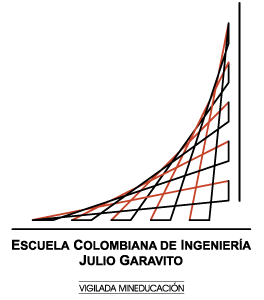
\includegraphics[scale=0.4]{University/escuela-logo.png}\\ % University/department logo - uncomment to place it
{\large \textrm{\today}}\\%[4cm] % Date
 
\vfill
\end{center}
\end{titlepage}

%----------------------------------------------------------------------------------------
%	DECLARATION PAGE
%----------------------------------------------------------------------------------------

% \begin{declaration}
% \addchaptertocentry{\authorshipname} % Add the declaration to the table of contents
% \noindent I, \authorname, declare that this thesis titled, \enquote{\ttitle} and the work presented in it are my own. I confirm that:

% \begin{itemize} 
% \item This work was done wholly or mainly while in candidature for a research degree at this University.
% \item Where any part of this thesis has previously been submitted for a degree or any other qualification at this University or any other institution, this has been clearly stated.
% \item Where I have consulted the published work of others, this is always clearly attributed.
% \item Where I have quoted from the work of others, the source is always given. With the exception of such quotations, this thesis is entirely my own work.
% \item I have acknowledged all main sources of help.
% \item Where the thesis is based on work done by myself jointly with others, I have made clear exactly what was done by others and what I have contributed myself.\\
% \end{itemize}
 
% \noindent Signed:\\
% \rule[0.5em]{25em}{0.5pt} % This prints a line for the signature
 
% \noindent Date:\\
% \rule[0.5em]{25em}{0.5pt} % This prints a line to write the date
% \end{declaration}

% \cleardoublepage

%----------------------------------------------------------------------------------------
%	QUOTATION PAGE
%----------------------------------------------------------------------------------------

% \vspace*{0.2\textheight}

% \noindent\enquote{\itshape Thanks to my solid academic training, today I can write hundreds of words on virtually any topic without possessing a shred of information, which is how I got a good job in journalism.}\bigbreak

% \hfill Dave Barry

%----------------------------------------------------------------------------------------
%	ABSTRACT PAGE
%----------------------------------------------------------------------------------------

% \begin{abstract}
% \addchaptertocentry{\abstractname} % Add the abstract to the table of contents
% In document language ...
% \end{abstract}

% \begin{extraAbstract}
% In english....
% \end{extraAbstract}

%----------------------------------------------------------------------------------------
%	ACKNOWLEDGEMENTS
%----------------------------------------------------------------------------------------

% \begin{acknowledgements}
% \addchaptertocentry{\acknowledgementname} % Add the acknowledgements to the table of contents
% The acknowledgments and the people to thank go here, don't forget to include your project advisor\ldots
% \end{acknowledgements}

%----------------------------------------------------------------------------------------
%	LIST OF CONTENTS/FIGURES/TABLES PAGES
%----------------------------------------------------------------------------------------

\tableofcontents % Prints the main table of contents

\listoffigures % Prints the list of figures

\listoftables % Prints the list of tables

%----------------------------------------------------------------------------------------
%	ABBREVIATIONS
%----------------------------------------------------------------------------------------

% \begin{abbreviations}{ll} % Include a list of abbreviations (a table of two columns)

% \textbf{LAH} & \textbf{L}ist \textbf{A}bbreviations \textbf{H}ere\\
% \textbf{WSF} & \textbf{W}hat (it) \textbf{S}tands \textbf{F}or\\

% \end{abbreviations}

%----------------------------------------------------------------------------------------
%	PHYSICAL CONSTANTS/OTHER DEFINITIONS
%----------------------------------------------------------------------------------------

% \begin{constants}{lr@{${}={}$}l} % The list of physical constants is a three column table

% % The \SI{}{} command is provided by the siunitx package, see its documentation for instructions on how to use it

% Speed of Light & $c_{0}$ & \SI{2.99792458e8}{\meter\per\second} (exact)\\
% %Constant Name & $Symbol$ & $Constant Value$ with units\\

% \end{constants}

%----------------------------------------------------------------------------------------
%	SYMBOLS
%----------------------------------------------------------------------------------------

% \begin{symbols}{lll} % Include a list of Symbols (a three column table)

% $a$ & distance & \si{\meter} \\
% $P$ & power & \si{\watt} (\si{\joule\per\second}) \\
% %Symbol & Name & Unit \\

% \addlinespace % Gap to separate the Roman symbols from the Greek

% $\omega$ & angular frequency & \si{\radian} \\

% \end{symbols}

%----------------------------------------------------------------------------------------
%	DEDICATION
%----------------------------------------------------------------------------------------

% \dedicatory{For/Dedicated to/To my\ldots} 

%----------------------------------------------------------------------------------------
%	THESIS CONTENT - CHAPTERS
%----------------------------------------------------------------------------------------

\mainmatter % Begin numeric (1,2,3...) page numbering

\pagestyle{thesis} % Return the page headers back to the "thesis" style

% Include the chapters of the thesis as separate files from the Chapters folder
% Uncomment the lines as you write the chapters

%----------------------------------------------------------------------------------------

% Define some commands to keep the formatting separated from the content 
\newcommand{\keyword}[1]{\textbf{#1}}
\newcommand{\tabhead}[1]{\textbf{#1}}
\newcommand{\code}[1]{\texttt{#1}}
\newcommand{\file}[1]{\texttt{\bfseries#1}}
\newcommand{\option}[1]{\texttt{\itshape#1}}

% ----------------------------------------------------------------------------------------

\chapter{Introducción} % Main chapter title

\label{chIntroduction} % For referencing the chapter elsewhere, use \ref{Chapter1} 

%----------------------------------------------------------------------------------------

\section{Objetivo general}
El objetivo de este proyecto es generar herramientas y estrategias para el perfilado de cibercriminales con ayuda de metodologías de \gls{nlp} aplicado a datos recolectados de fuentes abiertas por medio de \gls{osint}.

\section{Objetivos específicos}
\begin{enumerate}
\item Realizar minería de datos de fuentes abiertas de manera automatizada por medio de artefactos previamente construidos en \cite{osint}.
  
\item Explorar modelos de perfilamiento por medio de \glsentryfirst{kbs}, \glsentryfirst{bow} y \glsentryfirst{deepl} realizando una comparativa.

\end{enumerate}

\chapter{Cronograma} % Main chapter title

\label{ch:Schedule} % For referencing the chapter elsewhere, use \ref{Chapter1} 

%----------------------------------------------------------------------------------------

% \thispagestyle{empty}
\setcounter{taskcounter}{0}
\begin{figure}[h!]
  
\begin{tikzpicture}
    \GanttHeader{\textwidth}{2ex}{5cm}{16}
    \Taske{0}{5}{Entendimiento de \glsentrytext{osint}}
    \Taske{1}{9}{Estudio de literatura de \gls{nlp}}
    \Taske{2}{6}{Investigación del Estado del Arte}
    \Taske{6}{9}{Desarrollo de propuesta}
    \Taske{6}{9}{Implementación de software}
    \Taske{8}{6}{Profundización literatura de \gls{nlp}}
    \Taske{14}{2}{Preparación de documentos}
  \end{tikzpicture}
  \caption{Diagrama Gantt de actividades de 1\textsuperscript{er} periodo}
  \label{fig:gantt1}
\end{figure}


\setcounter{taskcounter}{0}
\begin{figure}[h!]
  
\begin{tikzpicture}
    \GanttHeader{\textwidth}{2ex}{5cm}{16}

    \Taske{0}{3}{Terminación de software P1}
    \Taske{0}{8}{Profundización en \gls{nlp}}
    \Taske{3}{3}{Desarrollo de técnicas de \glsentrytext{osint}}
    \Taske{6}{3}{Visualización de métodos}
    \Taske{9}{3}{Desarrollo de métodos adicionales}
    \Taske{12}{3}{Pruebas de concepto}
    \Taske{14}{2}{Documentación de documentos}
  \end{tikzpicture}
  \caption{Diagrama Gantt de actividades de 2\textsuperscript{do} periodo (Planeado)}
  \label{fig:gantt2}
\end{figure}

\vspace{1cm}

\newcounter{tablecountone}
\newcounter{tablecounttwo}
\setcounter{tablecountone}{1}
\setcounter{tablecounttwo}{0}
\newcommand{\rowt}[1]{\addtocounter{tablecounttwo}{1}{\thetablecountone.\thetablecounttwo} & {#1.} \\ \hline}
\newcommand{\tablenextlevel}{\addtocounter{tablecountone}{1}\setcounter{tablecounttwo}{0}}

\begin{table}[h!]
\begin{center}
\begin{tabular}{|c p{.975\textwidth}|} \hline
  \textbf{\#} & \textbf{Descripción} \\ \hline \hline
  
  \rowt{Entendimiento proyecto de \gls{osint}}
  \rowt{Estudio de la literatura de \gls{nlp}}
  \rowt{Investigación del Estado del Arte}
  \rowt{Desarrollo de la propuesta de investigación}
  \rowt{Desarrollo de la implementación y pruebas}
  \rowt{Realización de curso de \gls{nlp} de \emph{National Research University Higher School of Economics} en \gls{coursera}}
  \rowt{Preparación final de documento de libro de proyectos del primer periodo}
  % ================ SEGUNDO PERIODO ================
  \tablenextlevel
  \rowt{Terminación y mejora de software desarrollado en el primer periodo}
  \rowt{Periodización de metodologías aplicadas de \gls{nlp}}
  \rowt{Desarrollo de nuevas técnicas para la obtención de información de fuentes \glsentrytext{osint} como también de identificar nuevas fuentes de información que tengan que ver con terroristas}
  \rowt{Desarrollo de un \emph{dashboard} detallado que ayuden al agente de seguridad realizar sus labores}
  \rowt{Desarrollo de métodos adicionales para el perfilamiento de cibercriminales}
  \rowt{Realizar pruebas demostrativas que permitan visualizar la obtención de información de las fuentes abiertas en tiempo real}
  \rowt{Documentación final de los documentos entregables}
\end{tabular}
\end{center}
\caption{Detalle de cronograma de actividades}
\label{table:schedule}
\end{table}
 
\chapter{Marco teórico} % Main chapter title

\label{ch:MarcoTeorico} % For referencing the chapter elsewhere, use \ref{Chapter1} 

%----------------------------------------------------------------------------------------


La Web contiene una gran cantidad de opiniones respecto a productos, políticos, y mucho mas, expresado en forma de noticias, sitios de opinión, reseñas en tiendas online, redes sociales. Como resultado, el problema de ``Minería de opinión'' ha obtenido una atención creciente en las ultimas dos décadas y es un factor decisivo para las nuevas organizaciones (como es mencionado en \cite{Popescu2007}). De esto mismo partimos que el análisis de textos para extraer el significado y demás componentes extraíbles del texto componen un factor que debe considerarse al momento de realizar decisiones, de manera que los avances hechos hasta ahora tienen como meta una aplicación practica de lo que se conoce como \glsentrylong{nlp}.

Luego de los ataques terroristas del 11 de Septiembre de 2001 en Estados Unidos, se realizaron fuertes criticas respecto a la inteligencia, donde el director del FBI llamado \mbox{\emph{Robert~S.~Mueller}} indico que el principal problema que la agencia tuvo fue que se enfocaba demasiado en lidiar con el crimen luego de que fue cometido y ponía muy poco énfasis en prevenirlo (adaptado de \cite{mena2003investigative}). Es por esto que el uso de \gls{nlp} para temas de seguridad como también de metodologías de \glsentrylong{machinel} y \glsentrylong{deepl} han sido ampliamente utilizadas en ámbito de seguridad luego de estos eventos.

Para obtener una mejor inteligencia se necesito de mejores tecnologías a las que se tenían entonces (véase \cite[p\'ag 2]{mena2003investigative}):
\begin{itemize}
\item Integración de datos (o \gls{dataintegration} en ingles)
\item Análisis de vínculos (o \gls{linkanalisys} en ingles)
\item Agentes de software (o \gls{softwareagents} en ingles)
\item Minería de texto (o \gls{textmining} en ingles)
\item Redes neuronales (o \gls{neuralnetwork} en ingles)
\item Algoritmos de \glsentrylong{machinel} (o \gls{mlalgorithms} en ingles)
\end{itemize}

% ================================================================

\section{Análisis de vínculos (\glsentrylong{linkanalisys})}
Es la visualización de asociaciones entre entidades y eventos, por lo general involucran una visualización por medio de una gráfica o un mapa que muestre las relaciones entre sospechosos y ubicaciones, sea por medio físico o por comunicaciones en la red.

% ================================================================

\section{Agentes de software (\glsentrylong{softwareagents})}
Es el software que realiza tareas asignadas por el usuario de manera autónoma, donde sus habilidades básicas son:
\begin{itemize}
\item \textbf{Realización de tareas:} Hacen obtención de información, filtrado, monitoreo y reporte.
\item \textbf{Conocimiento:} Pueden usar reglas programadas, o pueden aprender reglas nuevas (véase \ref{sec:KBS}).
\item \textbf{Habilidades de comunicación:} Reportar a humanos e interactuar con otros agentes.
\end{itemize}

% ================================================================

\section{Aprendizaje de maquina (\glsentrylong{machinel})} \label{sec:ML}
De acuerdo con \cite{murphymachinel}, se define como un conjunto de métodos que pueden detectar patrones automáticamente en datos, y luego usar los patrones descubiertos para predecir los datos futuros, o realizar otra clase de toma de decisiones con un grado de incertidumbre, por tal motivo es necesario el uso de teoría de probabilidad, que puede ser aplicada a cualquier tipo de problema que involucra incertidumbre.

\subsection{Tipos de \glsentrylong{machinel}}
\gls{machinel} esta principalmente dividida en dos tipos. El método predictivo o bien \textbf{aprendizaje supervisado} (\gls{supervisedl}), donde el objetivo es aprender un mapeo de las entradas $\vx$ a las salidas $y$, dado un conjunto de pares de etiquetas de entrada--salida $D = \{(\vx_i, y_i)\}_{i=1}^{N}$. $D$ se le llama el conjunto de entrenamiento y $N$ es el numero de muestras de entrenamiento.

En la forma mas sencilla, cada entrada de entrenamiento $\vx_i$ es un vector $D$--dimensional de números, a estos se le llaman \emph{características} o \emph{atributos}.

De manera similar la forma de la salida puede ser en principio cualquier cosa, pero la mayoría de métodos asumen que $y_i$ es una variable \emph{categórica} o \emph{nominal} de algún conjunto finito, $y_i \in \{1,\ldots,C\}$, o que $y_i$ es un escalar real, $y_i \in \R$. Cuando la variable $y_i$ es categórica, al problema se le reconoce como \textbf{clasificación} o \textbf{reconocimiento de patrones}, y cuando es un valor real se le conoce como un problema de \textbf{regresión}.

El segundo tipo principal de \gls{machinel} es el descriptivo o \textbf{aprendizaje no--supervisado} (\gls{unsupervisedl}), en este solo están disponibles los datos de entrada $D = \{\vx_i\}_{i=1}^{N}$, y la meta es encontrar ``patrones interesantes'' en los datos. Este es un problema mucho menos definido, debido a que no se conocen los tipos de patrones que se quieren encontrar, y no hay una métrica obvia de error (no como aprendizaje supervisado en la que se puede comparar nuestra predicción de $y$ para un $\vx$ con el valor observado).

Un tercer tipo de aprendizaje de maquina es conocido como \textbf{\gls{reinforcedl}}, el cual es un tipo menos usado. Este es útil cuando se quiere aprender como actuar o comportarse cuando se recibe una recompensa ocasional o una señal de castigo.

\subsection{Sistemas de Detección de Anomalías (\glsentrylong{anomalydetectionsys})}
Existen diferentes aproximaciones para los sistemas de anomalías, sin embargo una similitud entre todos estos sistemas es que se intenta realiza una \emph{detección de desviaciones}, y su tarea es detectar los datos \emph{atípicos} en un sistema \cite{tan2005introduction}.

Uno de los que se pueden encontrar en la literatura son los sistemas de detección de anomalías basados en realizar un estimado probabilístico con alguna distribución de probabilidad de donde para una serie de características $m$ se trata de estimar una distribución gaussiana $X \sim \mathcal{N}(\mu, \sigma^2)$ que tiene media $\mu$ y varianza $\sigma^2$ por cada característica, por lo que existirán $m$ diferentes distribuciones .

Para estimar cada una las medias y variaciones de cada característica $j$, $\mu$ se estima con la \equationref{eq:anomaly-mu} y $\sigma^2$ se estima con la \equationref{eq:anomaly-sigma}.

\begin{equation} \label{eq:anomaly-mu}
  \mu_j = \frac{1}{m} \sum_{i=1}^{m} x_j^{(i)}
\end{equation}

\begin{equation} \label{eq:anomaly-sigma}
  \sigma_j^2 = \frac{1}{m} \sum_{i=1}^{m} (x_j^{(i)} - \mu_j)^2
\end{equation}

De donde para calcular la probabilidad de que una muestra se trata de una anomalía se calcula la probabilidad $p(x)$, luego de que fueron estimadas las distribuciones de cada característica del conjunto de entrenamiento, por lo que se define un $\epsilon$ de manera heurística, de forma que se determina que una muestra anómala si $p(x) < \epsilon$, la \equationref{eq:anomaly-prob} representa cual es la probabilidad de una muestra $x$ con una distribución gaussiana.

\begin{equation} \label{eq:anomaly-prob}
  p(x) = \prod_{j=1}^{n}p(x_j, \mu_j, \sigma_j^2) = \prod_{j=1}^{n} \frac{1}{\sqrt{2\pi}\sigma} \text{exp}\Bigg( - \frac{(x_j-\mu_j)^2}{2\sigma_j^2}\Bigg)
\end{equation}

Si el modelo esta dando como resultado muchos falsos positivos, lo que se debe hacer es reducir $\sigma$.

Este método de sistemas de detección de anomalía también es brevemente tratada en \cite{osint} con una representación de hiper-planos, que es equivalente con este descrito.

% ================================================================
\section{Minería de datos (\glsentrylong{datamining})} \label{sec:datamining}
Según \cite{tan2005introduction}, la minería de datos se define como el proceso de descubrir información útil en repositorios grandes de datos. Las técnicas de minería de datos son desplegadas para limpiar grandes bases de datos para encontrar patrones nuevos y útiles que de lo contrario podrían permanecer desconocidos. También ofrecen capacidades para predecir la salida de observaciones futuras, tales como predecir si un cliente nuevo gastara mas de \$100 en una tienda.

No todas las tareas de descubrimiento de información son considerados como \gls{datamining}. Por ejemplo, realizar una consulta de campos individuales usando un sistema de base de datos o encontrar una pagina web por medio de una búsqueda en Internet son tareas relacionadas con \emph{adquisición de información}.

\subsection{Minería de texto (\glsentrylong{textmining})} \label{subsec:NLP}
Es un subcampo de Inteligencia Artificial conocida como \glsentrylong{nlp}, en donde las herramientas de minería de datos pueden capturar rasgos críticos del contenido de un documento basado en el análisis de sus características lingüísticas.

La mayoría de los crímenes son electrónicos por naturaleza, por lo que se dejan rastros textuales que investigadores pueden seguir y analizar. Estas se enfocan en el descubrimiento de relaciones en texto no--estructurado y pueden ser aplicados al problema de \emph{búsqueda} y \emph{localización de palabras clave}.

\subsection{Clasificación} \label{subsec:clasification}
Clasificación es la tarea de asignarle una de varias categorías predefinidas a objetos, y es una tarea que tiene una variedad extensa de aplicaciones. Ejemplos de esto se encuentran la detección de correos no deseados en mensajes de e--mails basándose del encabezado o el cuerpo del mensaje, categorización de células benignas de malignas basándose en los resultados de escaneados MRI o incluso la clasificación de galaxias basado en su forma.

Definido formalmente, clasificación es la tarea de aprender una función objetivo $f$ que mapea cada conjunto de atributos $x$ a una clase predefinida de etiquetas $y$.

La función objetivo también se define informalmente como un \emph{modelo de clasificación}.

\subsubsection{Metodologías de clasificación} \label{subsubsec:classmethods}
Existen muchos métodos para la clasificación de datos no--estructurados, entre los descritos aquí están:
\begin{itemize}
\item Clasificador basado en reglas (véase la \sectionref{sec:KBS})
\item Redes neuronales artificiales (véase la \sectionref{sec:ANN})
\item Maquinas de soporte vectorial (véase la \sectionref{sec:SVM})
\item Clasificador de Na\"{\i}ve Bayes (véase la \sectionref{subsec:naivebayes})
\end{itemize}

\subsection{Clustering} \label{subsec:clustering}
El análisis de clusters agrupa objetos de datos basándose únicamente en la información encontrada en los datos que describen los objetos y sus relaciones. El objetivo es que objetos dentro de un grupo sean similares (o relacionados) el uno al otro, y que sean diferentes (o sin relación) a objetos en otros grupos. Entre mayor sea la similitud dentro de un grupo y entre mayor sea la diferencia entre grupos, sera mejor o mas distintivo el clustering.

Los métodos de clustering se hacen referencia comúnmente en \gls{machinel} como métodos no--supervisados, los cuales se describen en \ref{sec:ML}. Un método de estos se describe en \ref{subsec:SOM} conocidos como mapas autoorganizados.

% ================================================================

\section{Sistemas Basados en Conocimiento (\glsentrylong{kbs})} \label{sec:KBS}
Según \cite{sajja2010knowledge}, los \gls{kbs} son uno de los mayores miembros de la familia de \gls{ai}. El \gls{kbs} consiste de una \gls{knowledgebase} y un programa de búsqueda llamado \gls{inferenceengine} representado en la \figureref{fig:kbs-arch}. La \gls{knowledgebase} puede ser usado como un repositorio de conocimiento de varias formas.

Existen 5 tipos de \gls{kbs}, donde uno de ellos es conocido como \gls{expertsystems}, usados como \gls{rulebasedsys}, donde su \gls{knowledgebase} esta dado como reglas y el \gls{inferenceengine} esta dado por algo llamado \gls{workingmemory}, que representa los hechos que se conocen inicialmente del sistema junto con los hechos que se van dando como inferencia de las reglas.

\begin{figure}[H]
\centering
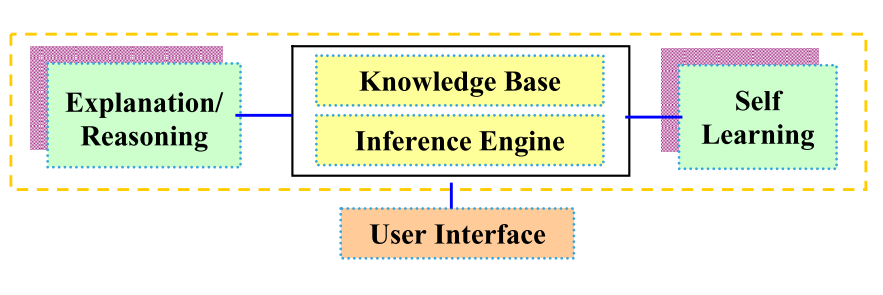
\includegraphics[scale=0.4]{Figures/kbs-architecture.png}
\decoRule
\caption[Arquitectura \glsentrytext{kbs}]{Arquitectura \glsentrytext{kbs}. Tomado de \cite{sajja2010knowledge}}
\label{fig:kbs-arch}
\end{figure}

Estas reglas pueden resumirse como una colección de condicionales de la forma \textbf{IF/ELSE} que se componen de un \emph{antecedente} y un \emph{consecuente}.

Existen dos tipos de \gls{rulebasedsys}, definidos como \gls{deductivesys} y \gls{reactivesys}, donde el \gls{deductivesys} tiene como objetivo realizar una conclusión en base a los hechos iniciales en la \gls{workingmemory}, por el otro lado se tienen los \gls{reactivesys}, los cuales de igual manera a los \gls{deductivesys}, toman los hechos de la \gls{workingmemory} y realizan sea una acción interactiva con su entorno o bien una modificación de los hechos que se encuentran en la \gls{workingmemory} tal como la adición o eliminación de hechos. Tómese el ejemplo de la \equationref{eq:rbs-example} tomada de \cite{Mendel}, donde \emph{x} es la temperatura y \emph{AC} es aire acondicionado.

\begin{equation} \label{eq:rbs-example}
  \left\{ \begin{array}{ll}
            \text{IF x es moderado,} & \text{THEN y = ajustar AC a bajo} \\
            \text{IF x es alto,}     & \text{THEN y = ajustar AC a moderado a alto} \\
            \text{IF x es muy alto,} & \text{THEN y = ajustar AC a alto} 
          \end{array} \right.
\end{equation}

% ================================================================

\section{Redes Neuronales Artificiales (\glsentrylong{neuralnetwork})} \label{sec:ANN}
El estudio de redes neuronales artificiales fue inspirado por los intentos de simular los sistemas biológicos de neuronas. El cerebro humano se compone principalmente de células nerviosas llamadas \emph{neuronas}, enlazadas con otras neuronas por medio de hebras de fibra conocidas como \emph{axones}. Los axones son usados para transmitir impulsos nerviosos de una neurona a otra cada vez que las neuronas son estimuladas. Una neurona esta conectada a axones de otras neuronas por medio de \emph{dendritas}, las cuales son extensiones desde el cuerpo de la neurona. El punto de contacto entre una dendrita y un axón se conoce como \emph{sinapsis}. Los neurólogos han descubierto que el cerebro humano aprende por medio de cambiar la fuerza de la conexión sináptica entre las neuronas a través de estimulación repetitiva por el mismo impulso.

De manera análoga a la estructura del cerebro humano, una \gls{neuralnetwork} se compone de una estructura interconectada de nodos y vínculos directos.

\subsection{Mapa autoorganizado (\glsentrylong{som})} \label{subsec:SOM}
El objetivo principal de los \gls{som} es de transformar una patrón de entrada $m$--dimensional en un mapa discreto uni-- o bi--dimensional, donde sus principales características es que es un algoritmo que se basa en \gls{unsupervisedl}, es \gls{feedforward}, tiene una sola capa de neuronas donde su propósito es realizar \gls{clustering} y una reducción de dimensionalidad sobre los datos de una forma topológicamente ordenada.

Los \gls{som} tienen tres características distintivas:
\begin{itemize}
\item {\bf Competencia:} por cada patrón de entrada, las neuronas en la red competirán entre ellas para determinar un ganador.
\item {\bf Cooperación:} la neurona ganadora determina la ubicación espacial (vecinos) alrededor de donde otras vecinas también se verán estimuladas.
\item {\bf Adaptación:} la neurona ganadora como también sus vecinas tendrán sus pesos asociados actualizados, y se tiene que los vecinos entre mas cerca estén del ganador, mayor es el grado de adaptación.
\end{itemize}

El algoritmo de aprendizaje de \gls{som} parte de primero inicializar los pesos de las $o$ neuronas con pesos aleatorios pequeños de una distribución de probabilidad aleatoria o uniforme, donde cada vector de entrada se define como $\vx = [x_1, \ldots, x_m]^{\top} \in \R^{m}$ y la entrada general de $N$ patrones como $\mX^{m \times N}$, el vector de pesos de la neurona $i$ es $\vw_i = [w_{i1}, \ldots, w_{im}] \in \R^{1 \times m}$, con la matriz de pesos $\mW^{o \times m}$.

Para alcanzar el objetivo de \emph{competencia}, se realiza por cada patrón de entrada $x_i$ una comparación con cada uno de los pesos de las $o$ neuronas y se establece la de menor distancia $\norm{x_i}_p$ (típicamente la distancia Euclidiana o equivalentemente la norma $\normltwo$ e.g. $p = 2$), dejando un ganador $winner$, tal como en la \equationref{eq:som-competition}.
\begin{equation} \label{eq:som-competition}
  winner = \text{argmin}_j \norm{x_i - w_j}_p ; j = 1, \ldots,o
\end{equation}

Luego de establecer la neurona ganadora, se realiza el paso para alcanzar la \emph{cooperación}, que consiste en que por medio de una función kernel $h$ (típicamente una una distribución gaussiana), que permite establecer un área de afectación de las otras neuronas según su ubicación física en el mapa, definidos como $r_{winner}$ y $r_j$ que son la ubicación de la neurona ganadora y la neurona vecina $j$, en el cual el grado de afectación de la neurona vecina depende de la distancia $\normltwo$ de la que esta de la neurona ganadora, definido en la \equationref{eq:som-cooperation}.
\begin{equation} \label{eq:som-cooperation}
  h_{j, winner}(t) = \text{exp}\Bigg(\frac{- \norm{r_j - r_{winner}}^2}{ 2 \sigma(t)^2}\Bigg)
\end{equation}

Parte importante del proceso de convergencia del \gls{som} es que a medida que avanzan las iteraciones $t$ del algoritmo el área de afectación se va reduciendo como parte del proceso de adaptación, por lo que definimos $\sigma(t) = \sigma_0 \text{exp}(-t / \tau_1)$, donde $\tau_1$ es una constante heurística y $\sigma_0$ la dimensión del mapa \gls{som}.

Finalmente para alcanzar la \emph{adaptación} se realiza una actualización de los pesos de la matriz $\mW$ en base a la influencia de área $\sigma(t)$ y de una tasa de aprendizaje $\lr(t) = \lr_0 \text{exp}(-t/ \tau_2)$, donde $\tau_2$ es otra constante heurística y $\lr_0$ es una constante de aprendizaje inicial, que debe ser $0 \le \lr_0 \le 1$, la actualización se describe por la \equationref{eq:som-adaptation} y el proceso puede ser visto gráficamente en la \figureref{fig:som-adap-proc}, tanto de forma uni-- como bi--dimensional.
\begin{equation} \label{eq:som-adaptation}
  w_j(t+1) = w_j(t) + \lr(t) h_{j, winner}(t)\Big[x_i-w_j(t)\Big]
\end{equation}

\begin{figure}[H]
\centering
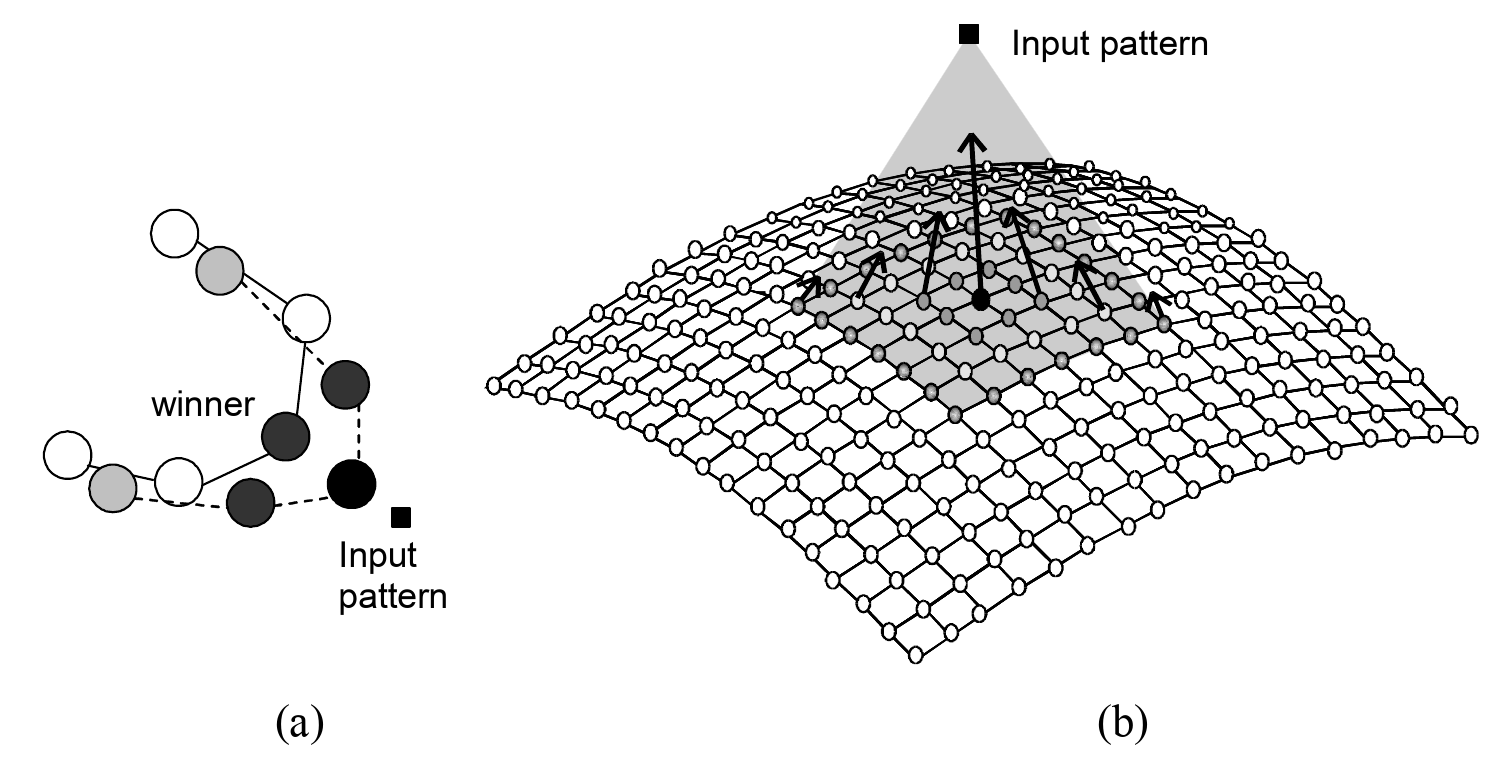
\includegraphics[scale=0.2]{Figures/som-adaptive-proc.png}
\decoRule
\caption[Proceso de adaptación de \glsentrytext{som}]{Proceso de adaptación de \glsentrytext{som}, (a) uni--dimensional, (b) bi--dimensional. Tomado de \cite{de2006fundamentals}}
\label{fig:som-adap-proc}
\end{figure}

Luego de que el algoritmo de aprendizaje termina de realizar las iteraciones, la salida de este es la matriz de pesos $\mW$, en la \figureref{fig:som-impl-example} se puede apreciar una aproximación del algoritmo con un mapa uni--dimensional tratando de aproximar una función sinusoidal con ruido adicionado en un gráfico 2D.

En la \figureref{fig:som-example} se puede ver una aplicación de los \gls{som}, en donde se realiza una clusterizacion de casos de homicidios donde los parametros son características de los homicidios, según \cite{mena2003investigative} este resultado da una buena aproximación para sospechar de que estos son cometidos por personas distintas o si bien están siendo perpetrados por un mismo individuo o grupo.

\todo{Cambiar grafica por otra, polar?}
\begin{figure}[H]
\centering
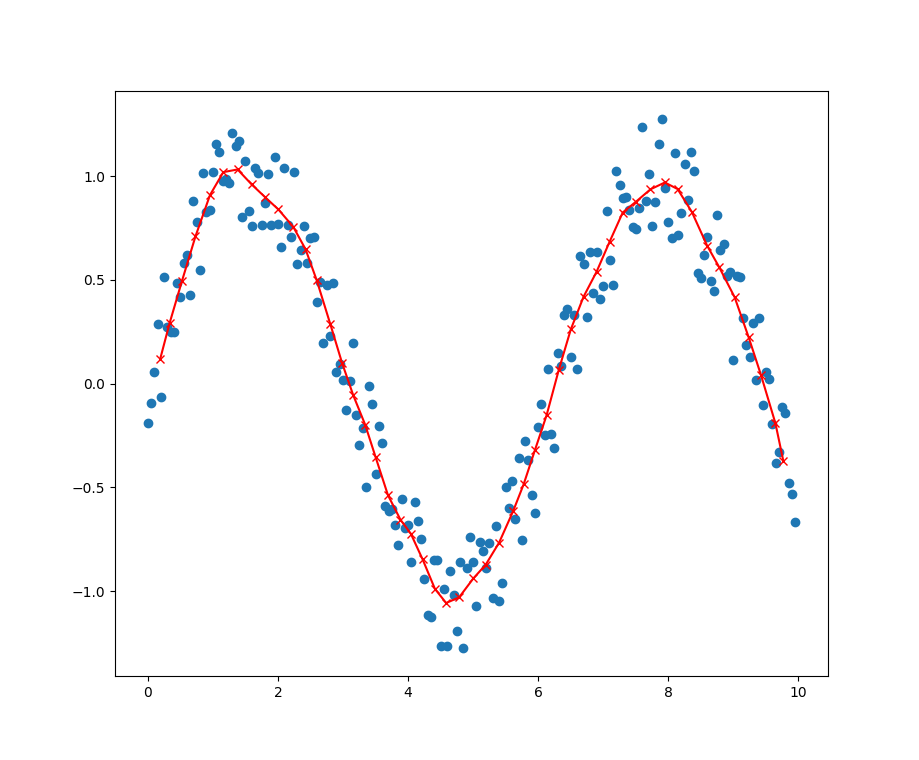
\includegraphics[scale=0.5]{Figures/som-implementation-example.png}
\decoRule
\caption[Ejemplo de salida de \glsentrytext{som} uni-dimensional]{Ejemplo de salida de \glsentrytext{som} uni-dimensional. Implementación propia.}
\label{fig:som-impl-example}
\end{figure}

\begin{figure}[H]
\centering
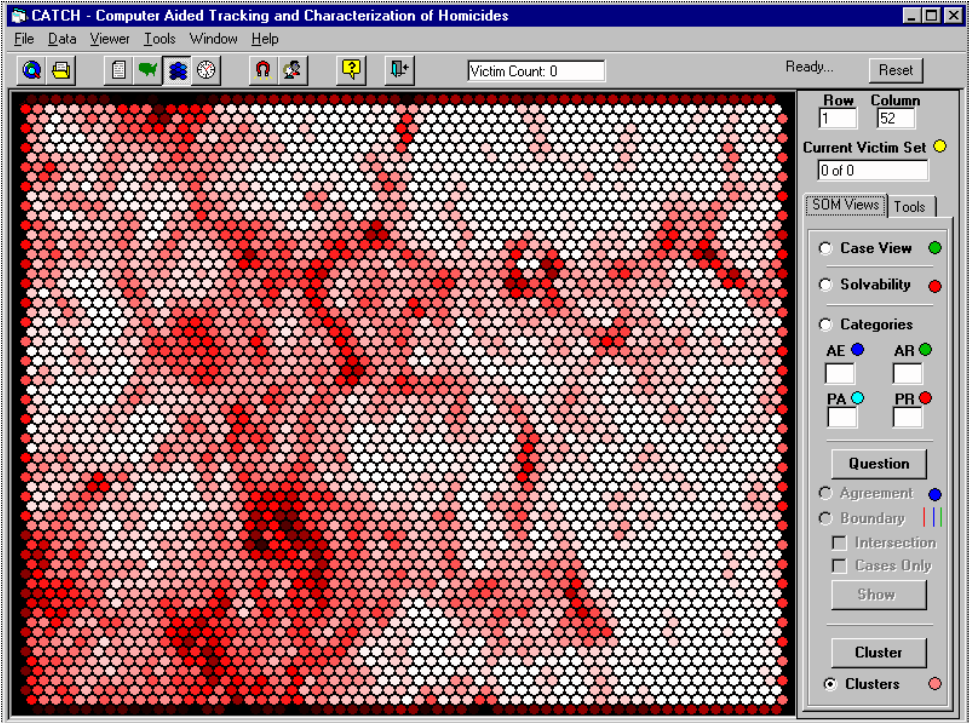
\includegraphics[scale=0.3]{Figures/som-example.png}
\decoRule
\caption[Ejemplo de uso de \glsentrytext{som} en aplicaciones de perfilado]{Ejemplo de uso de \glsentrytext{som} en aplicaciones de perfilado. Tomado de \cite{mena2003investigative}}
\label{fig:som-example}
\end{figure}

% ================================================================

\section{Maquina de soporte vectorial (\glsentrylong{svm})} \label{sec:SVM}
\gls{svm} es una técnica de clasificación que tiene sus raíces en la teoría de aprendizaje estadístico que ha mostrado resultados empíricos prometedores en muchas aplicaciones practicas, desde reconocimiento de dígitos escritos a mano a categorización de texto. \gls{svm} también funciona muy bien con datos de alta dimensionalidad. Otro aspecto destacable de esta aproximación es que representa la frontera de decisión usando un subconjunto de las muestras de entrenamiento, conocidos como los \emph{support vectors}.

\subsection{Maximum Margin Hyperplanes}
Se puede entender a los \gls{mmh} como hiper-planos que ayudan a separar datos en un hiper-espacio y que poseen un margen de decisión entre los datos, como ejemplo tómese la \figureref{fig:svm-hyperplanes}, donde el hiper-plano $B_1$ tiene un margen de decisión mas grande que el hiper-plano $B_2$.

\begin{figure}[H]
\centering
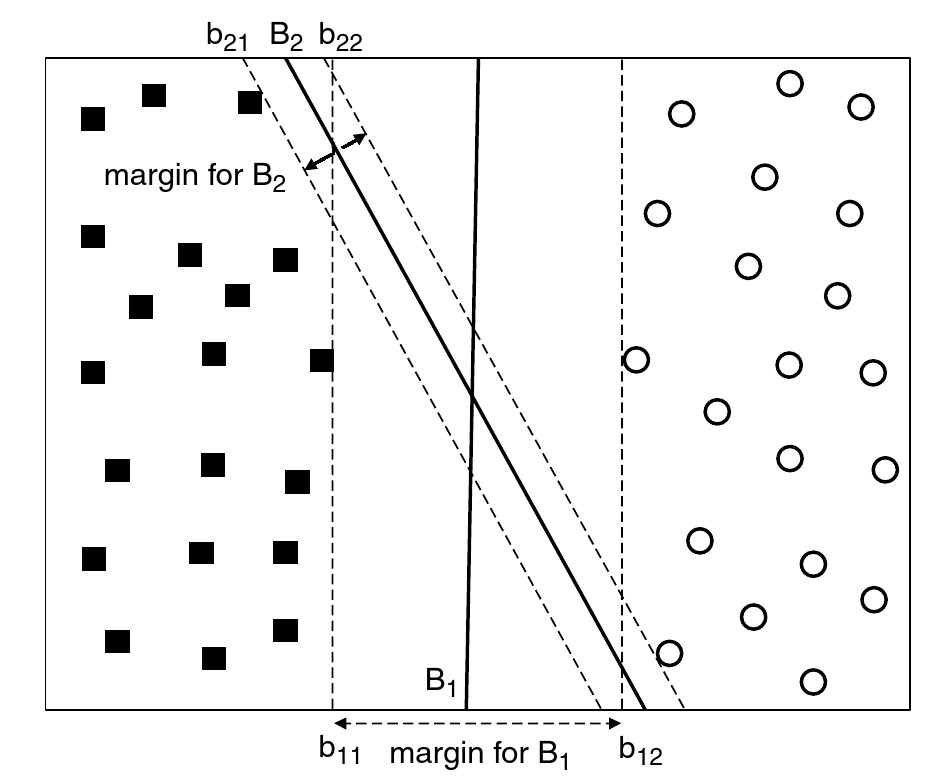
\includegraphics[scale=0.3]{Figures/svm-hyperplanes.png}
\decoRule
\caption[\glsentryname{mmh}]{\glsentryname{mmh}. Tomado de \cite{tan2005introduction}}
\label{fig:svm-hyperplanes}
\end{figure}

Finalmente, el objetivo final de los \gls{svm} es la búsqueda de un hiper-plano con el mayor margen de decisión. Existen dos tipos de \gls{svm}, el lineal y el no--lineal. El lineal realiza la separación de los datos con su hiper-plano a partir de los datos de entrada en su espacio vectorial original, mientras que el no--lineal consta de realizar una transformación de los espacios de los datos de entrada a uno en que sea linealmente separable (véase como ejemplo la \figureref{fig:svm-nonlinear-transforms}), sin embargo al realizar la transformación, el algoritmo de \gls{svm} se ve afectado por la dimensionalidad de la entrada, por lo que existe lo que se conoce como la función \emph{kernel} para remediarlo.

\begin{figure}[H]
\centering
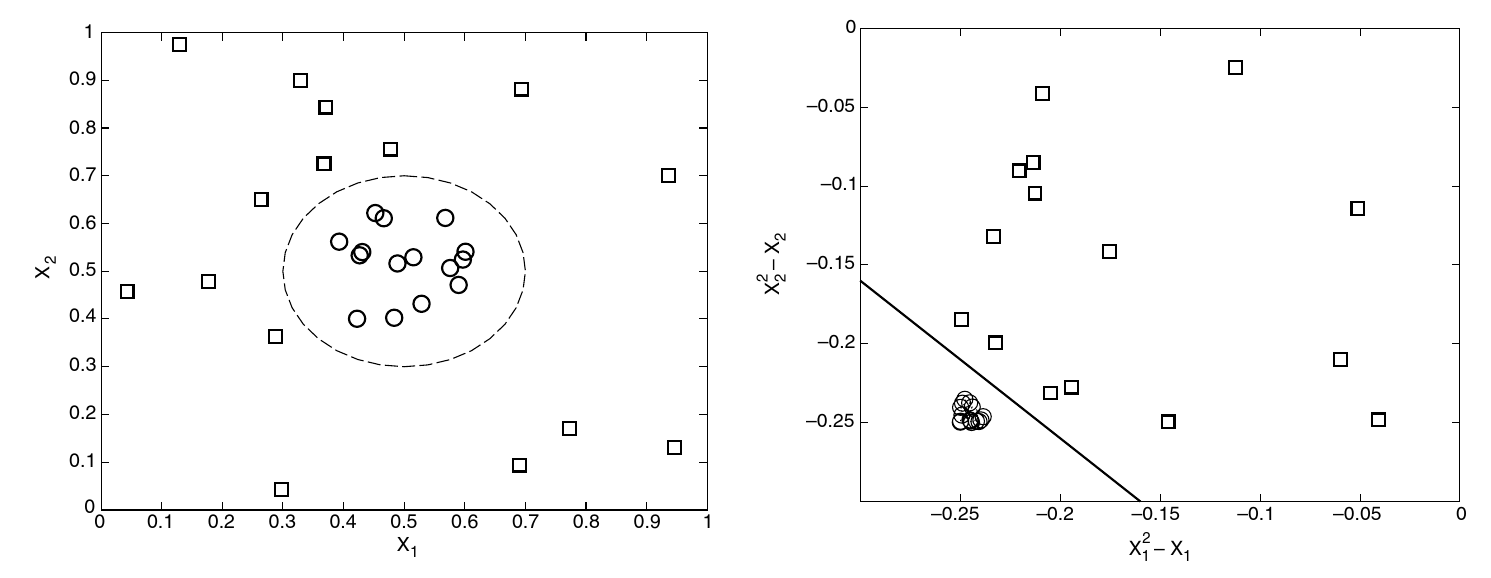
\includegraphics[scale=0.25]{Figures/svm-nonlinear-transform.png}
\decoRule
\caption[Transformación de espacios en \glsentrylong{svm}]{Transformación de espacios en \glsentrylong{svm}. Tomado de \cite{tan2005introduction}}
\label{fig:svm-nonlinear-transforms}
\end{figure}

\subsection{Función Kernel}
La función polinomial de similaridad, $K$, la cual es calculada en el espacio original de los datos de entrada, se le conoce como la \textbf{función Kernel}. En principio se asegura que la función kernel puede ser expresada siempre como el producto punto entre dos vectores de entrada en algún espacio de alta dimensionalidad, la función de kernel también tiene la particularidad de que el computo de los productos punto con la función toman considerablemente menos tiempo que realizar la transformación de espacios, dejando de lado la transformación, acelerando la tarea de clasificación.

% ================================================================

\section{Clasificadores Bayesianos} \label{sec:bayes}
En muchas aplicaciones de relaciones entre el conjunto de atributos y la etiqueta es no--determinante. Es decir, la etiqueta de clase de un dato de un conjunto de prueba no puede ser determinado con certeza a pesar de ser un atributo idéntico a los atributos de entrenamiento. Esto puede ser producto de que los datos poseen ruido o la presencia de ciertos factores que afectan la clasificación pero no son incluidos en el análisis. Para esto es crucial el teorema de Bayes, el cual es un principio estadístico que combina el conocimiento previo de las clases con la nueva evidencia que se obtiene de los datos.

\subsection{Teorema de Bayes} \label{subsec:bayestheo}
El teorema de Bayes dice que para un par de variables aleatorias $\rx$ e $\ry$, donde $P(\rx=x | \ry=y)$ es la probabilidad de que la variable $\rx$ tome el valor $x$ dado que el valor de la variable $\ry$ es $y$. Se tiene entonces la \equationref{eq:bayestheo}.
\begin{equation} \label{eq:bayestheo}
  P(\ry | \rx) = \frac{P(\rx | \ry) P(\ry)}{P(\rx)}
\end{equation}

\subsubsection{Usando el teorema de Bayes para clasificación}
Para denotar el problema de clasificación desde una perspectiva estadística se define a $\rx$ como el conjunto de atributos y $\ry$ como el conjunto de etiquetas de clase. Si la etiqueta de clase tiene una relación no--determinante con los atributos, entonces se pueden tomar a $\rx$ y a $\ry$ como variables aleatorias y capturar su relación probabilística con $P(\ry|\rx)$, conocida como la probabilidad posterior para $\ry$, dada su probabilidad previa $P(\ry)$.

Durante la fase de entrenamiento, es necesario aprender las probabilidades posteriores $P(\ry|\rx)$ para cualquier combinación de $\rx$ y $\ry$ basándose en la información recolectada de los datos de entrenamiento.

Dado que lo que se quiere realizar es una clasificación que represente la probabilidad de que dado un valor de $\rx=x$ este relacionado con que $\ry=y$, se puede reconocer primero que $\rx$ se mantiene constante para lo que son los datos de entrenamiento, y que lo desconocido sea la clasificación $\ry=y$ con probabilidad $P(\ry|\rx)$, al conocer esta probabilidad, un valor de prueba $\rx'$ puede ser clasificado por medio de encontrar la clase $\ry'$ que maximice la probabilidad posterior $P(\ry'|\rx')$.


\subsection{Clasificador Na\"{\i}ve Bayes} \label{subsec:naivebayes}
Un clasificador de Na\"{\i}ve Bayes estima la probabilidad condicional de las clases por medio de suponer que los atributos son condicionalmente independientes, dado la etiqueta de clasificación $y$. La suposición de independencia condicional se puede dar por la \equationref{eq:bayes-conditional-independence}.

\begin{equation} \label{eq:bayes-conditional-independence}
  P(X|\ry=y) = \prod_{i=1}^{d} P(\rx_i|\ry=y)
\end{equation}

Donde cada conjunto de atributos $X=\{ \rx_1, \ldots, \rx_d \}$ que consiste de $d$ atributos.
\subsubsection{Como funciona el clasificador Na\"{\i}ve Bayes}
Con la suposición de independencia condicional, en vez de computar la probabilidad condicional de clases para cada combinación de $X$, solo se debe realizar para establecer la probabilidad condicional de cada $\rx_i$, dado $\ry$.

Para clasificar un dato de prueba, el clasificador computa la probabilidad posterior para cada clase $\ry$ como se muestra en la \equationref{eq:bayes-classifier}.

\begin{equation} \label{eq:bayes-classifier}
  P(\ry|\rx) = \frac{P(\ry) \prod_{i=1}^{d}P(\rx_i|\ry)}{P(\rx)}
\end{equation}


\chapter{Estado del arte} % Main chapter title

\label{chStateOfTheArt} % For referencing the chapter elsewhere, use \ref{Chapter1} 

%----------------------------------------------------------------------------------------


La Web contiene una gran cantidad de opiniones respecto a productos, políticos, y mucho mas, expresado en forma de noticias, sitios de opinión, reseñas en tiendas online, redes sociales. Como resultado, el problema de ``Minería de opinión'' ha obtenido una atención creciente en las ultimas dos décadas y es un factor decisivo para las nuevas organizaciones (como es mencionado en \cite{Popescu2007}). De esto mismo partimos que el análisis de textos para extraer el significado y demás componentes extraíbles del texto componen un factor que debe considerarse al momento de realizar decisiones, de manera que los avances hechos hasta ahora tienen como meta una aplicación practica de lo que se conoce como \glsentrylong{nlp}.

Luego de los ataques terroristas del 11 de Septiembre de 2001 en Estados Unidos, se realizaron fuertes criticas respecto a la inteligencia, donde el director del FBI~\emph{Robert~S.~Mueller} indico que el principal problema que la agencia tuvo fue que se enfocaba demasiado en lidiar con el crimen luego de que fue cometido y ponía muy poco énfasis en prevenirlo. Es por esto que el uso de \gls{nlp} para temas de seguridad como también de metodologías de \glsentrylong{machinel} y \glsentrylong{deepl} han sido ampliamente utilizadas en ámbito de seguridad luego de estos eventos.

Para obtener una mejor inteligencia se necesito de mejores tecnologías a las que se tenían entonces (véase \cite[p\'ag 2]{mena2003investigative}):
\begin{itemize}
\item Integración de datos (\'o \gls{dataintegration} en ingl\'es)
\item Análisis de vínculos (\'o \gls{linkanalisys} en ingl\'es)
\item Agentes de software (\'o \gls{softwareagents} en ingl\'es)
\item Minería de texto (\'o \gls{textmining} en ingl\'es)
\item Redes neuronales (\'o \gls{neuralnetworks} en ingl\'es)
\item Algoritmos de \glsentrylong{machinel} (\'o \gls{mlalgorithms} en ingl\'es)
\end{itemize}

% ================================================================

\section{Análisis de vínculos (\glsentrylong{linkanalisys})}
Es la visualización de asociaciones entre entidades y eventos, por lo general involucran una visualización por medio de una gráfica o un mapa que muestre las relaciones entre sospechosos y ubicaciones, sea por medio físico o por comunicaciones en la red.

% ================================================================

\section{Agentes de software (\glsentrylong{softwareagents})}
Es el software que realiza tareas asignadas por el usuario de manera autónoma, donde sus habilidades básicas son:
\begin{itemize}
\item \textbf{Realización de tareas:} Hacen obtención de información, filtrado, monitoreo y reporte.
\item \textbf{Conocimiento:} Pueden usar reglas programadas, o pueden aprender reglas nuevas (véase \ref{secKBS}).
\item \textbf{Habilidades de comunicación:} Reportar a humanos e interactuar con otros agentes.
\end{itemize}

% ================================================================

\section{Sistemas Basados en Conocimiento (\glsentrylong{kbs})} \label{secKBS}
Según \cite{sajja2010knowledge}, los \gls{kbs} son uno de los mayores miembros de la familia de \gls{ai}. El \gls{kbs} consiste de una \gls{knowledgebase} y un programa de búsqueda llamado \gls{inferenceengine} representado en la figura \ref{fig:kbs-arch}. La \gls{knowledgebase} puede ser usado como un repositorio de conocimiento de varias formas.

Existen 5 tipos de \gls{kbs}, donde uno de ellos es conocido como \gls{expertsystems}, donde su uso se da como \gls{rulebasedsys}, donde su \gls{knowledgebase} esta dado como reglas y su \gls{inferenceengine} esta dado por algo llamado \gls{workingmemory}, que representa los hechos que se conocen inicialmente del sistema junto con los hechos que se van dando como inferencia de las reglas.

\begin{figure}[th]
\centering
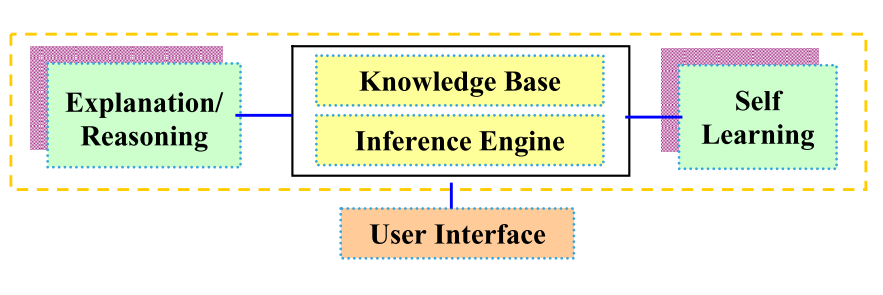
\includegraphics[scale=0.4]{Figures/kbs-architecture.png}
\decoRule
\caption[Arquitectura \glsentrytext{kbs}]{Arquitectura \glsentrytext{kbs}. Tomado de \cite{sajja2010knowledge}}
\label{fig:kbs-arch}
\end{figure}

Estas reglas pueden resumirse como una colección de condicionales de la forma \textbf{IF/ELSE} que se componen de un \emph{antecedente} y un \emph{consecuente}.

Existen dos tipos de \gls{rulebasedsys}, definidos como \gls{deductivesys} y \gls{reactivesys}, donde el \gls{deductivesys} tiene como objetivo realizar una conclusión en base a los hechos iniciales en la \gls{workingmemory}, por el otro lado se tienen los \gls{reactivesys}, los cuales de igual manera a los \gls{deductivesys}, toman los hechos de la \gls{workingmemory} y realizan sea una acción interactiva con su entorno o bien una modificación de los hechos que se encuentran en la \gls{workingmemory} tal como la adición o eliminación de hechos. Tómese el ejemplo de \ref{eq:rbs-example}, donde AC es aire acondicionado.

\begin{equation} \label{eq:rbs-example}
  \left\{ \begin{array}{rl}
            \text{IF x es moderado, THEN y = ajustar AC a bajo} \\
            \text{IF x es alto, THEN y = ajustar AC a moderado a alto} \\
            \text{IF x es muy alto, THEN y = ajustar AC a alto} 
          \end{array} \right.
\end{equation}

\subsection{Fuzzy Knowledge Based Systems}
Pendiente

% ================================================================

\section{Mineria de texto (\glsentrylong{textmining})} \label{secNLP}
Es un subcampo de Inteligencia Artificial conocida como \glsentrylong{nlp}, en donde las herramientas de minería de datos pueden capturar rasgos críticos del contenido de un documento basado en el análisis de sus características lingüísticas.

La mayoría de los crímenes son electrónicos por naturaleza, por lo que se dejan rastros textuales que investigadores pueden seguir y analizar.Estas se enfocan en el descubrimiento de relaciones en texto no--estructurado y pueden ser aplicados al problema de \emph{búsqueda} y \emph{localización de palabras clave}.

% ================================================================

\section{Redes Neuronales (\glsentrylong{neuralnetworks})} \label{secNN}
Pendiente

\subsection{Sistemas de Detección de Anomalías (\glsentrylong{anomalydetectionsys})}
Pendiente

\subsection{Mapa autoorganizado (\glsentrylong{som})}
Pendiente
\begin{figure}[th]
\centering
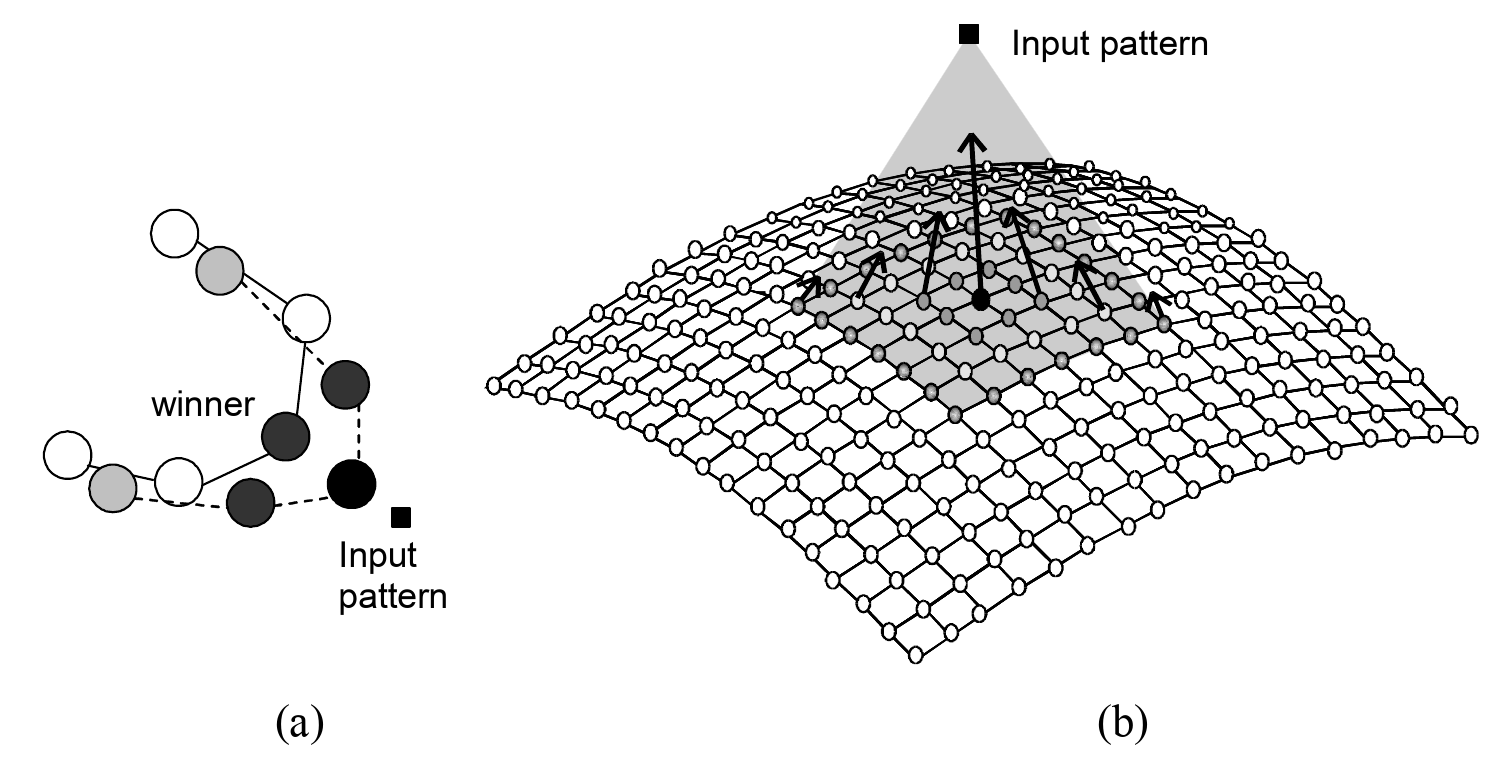
\includegraphics[scale=0.2]{Figures/som-adaptive-proc.png}
\decoRule
\caption[Proceso de adaptación de \glsentrytext{som}]{Proceso de adaptación de \glsentrytext{som}. Tomado de \cite{de2006fundamentals}}
\label{fig:som-adap-proc}
\end{figure}

\begin{figure}[th]
\centering
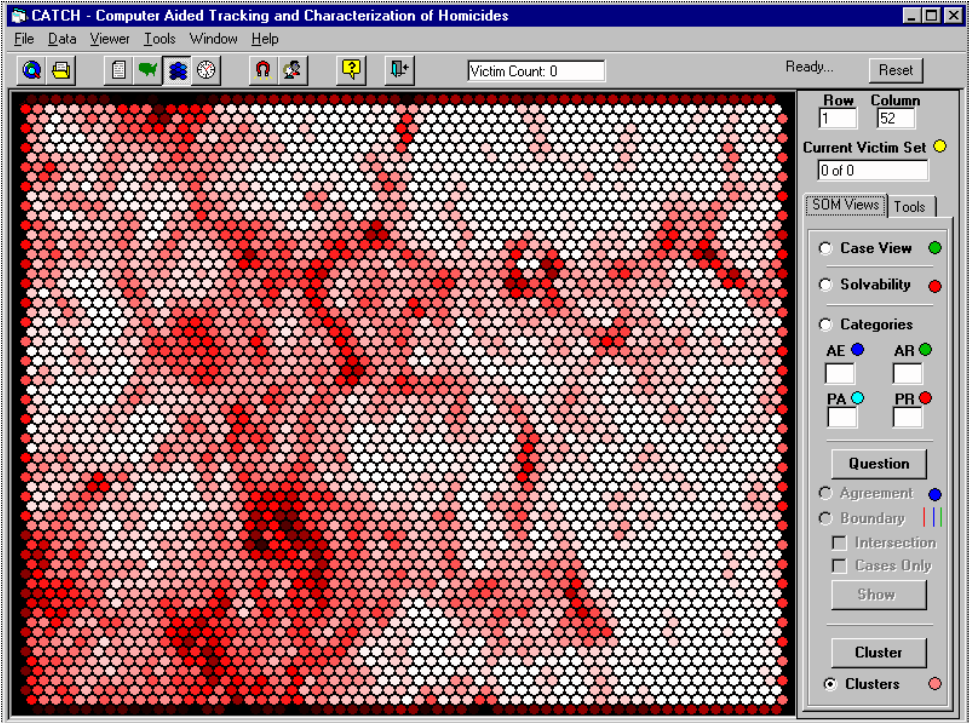
\includegraphics[scale=0.3]{Figures/som-example.png}
\decoRule
\caption[Ejemplo de uso de \glsentrytext{som}]{Ejemplo de uso de \glsentrytext{som}. Tomado de \cite{mena2003investigative}}
\label{fig:som-example}
\end{figure}

% ================================================================

\section{Aprendizaje de maquina (\glsentrylong{machinel})} \label{secML}
Pendiente
% Chapter 3

\chapter{Propuesta} % Main chapter title

\label{Chapter3} % For referencing the chapter elsewhere, use \ref{Chapter1} 

%----------------------------------------------------------------------------------------

\newcommand{\nmodels}{$n$ \todo{?`cuantos modelos?}}

La propuesta consta de \nmodels modelos, pensados para el análisis de texto en redes sociales como Twitter en aras de realizar un perfilado de ciber-criminales potenciales, esto por medio de \gls{nlp}, de donde se parte varias metodologías que hacen uso de tecnologías \mbox{Estado-del-Arte}.

\section{Análisis}
\todo{averiguar que se pone en esta sección}

\section{Diseño}
Como parte de la propuesta se proponen \nmodels modelos para tratar diferentes aspectos en perfilado de donde se representan los diferentes modelos en la \figureref{fig:proposal-arch}.

\begin{figure}[H]
  \centering
  \missingfigure{Hacer la arquitectura en yEd}
% 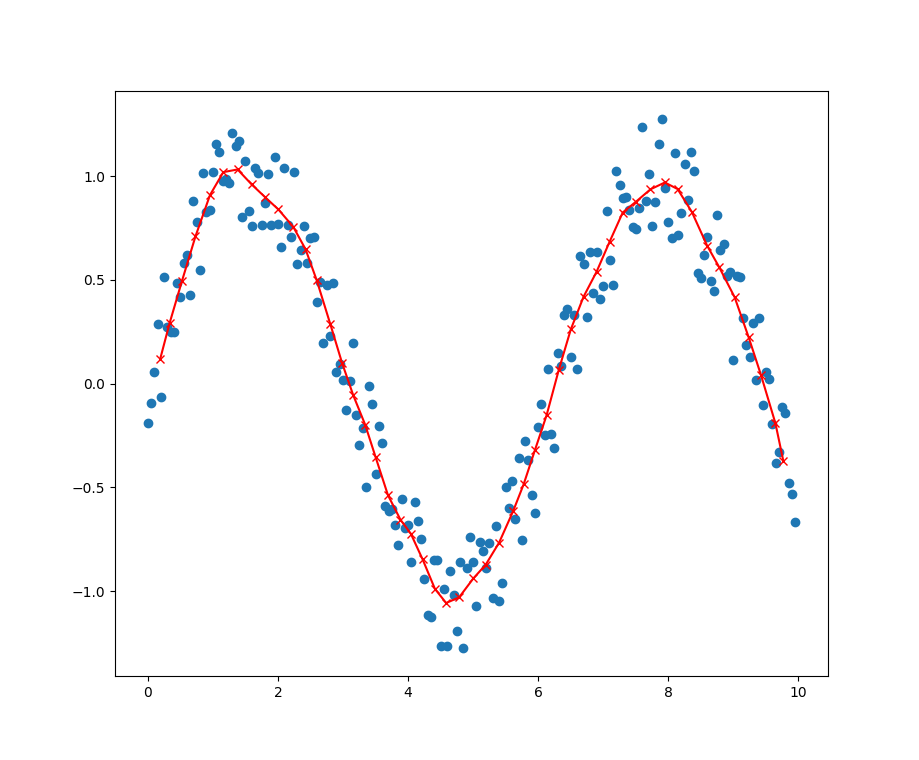
\includegraphics[scale=0.5]{Figures/som-implementation-example.png}
\decoRule
\caption[Arquitectura de propuesta]{Arquitectura de propuesta.}
\label{fig:proposal-arch}
\end{figure}

\subsection{Predicción de etiquetas de Twitter con modelos lineales}
En Twitter, las publicaciones que se realizan tienen la posibilidad de incluir menciones de temas de tendencia por el conocido \emph{hashtag}, escrito como \texttt{\#Tema}, y tiene la gran utilidad de realizar una mención explicita del tema que se quiere tratar y donde además la tarea de encontrar textos directamente relacionados con un tema son fácilmente localizables.

Así mismo, en la literatura de \gls{nlp} es muy común el uso de diferentes representaciones de palabras o conjuntos de palabras. Una representación de palabras típicas es por medio de los \gls{bow}, donde se establece un diccionario de palabras de tamaño $N$, y donde cada palabra tiene un vector que lo representa. A cada palabra se le asigna un identificador único en ese diccionario, por lo que existiría una traducción de palabra a identificador y una secuencia de palabras para poder ser recuperado por medio del índice, como se muestra en la \equationref{eq:bow-repr1} y la \equationref{eq:bow-repr2}.
\begin{equation} \label{eq:bow-repr1}
  \text{word2idx} = \Big\{(\text{word}_i, i) : \forall i \in [1, \ldots, N] \Big\}
\end{equation}

\begin{equation} \label{eq:bow-repr2}
  \text{idx2word} = \Big[\text{word}_i\Big], \forall i \in [1, \ldots, N]
\end{equation}

Otra representación común en \gls{nlp} es la de \gls{tfidf}, que se divide en dos partes, expresadas en las \equationref{eq:tf-repr}, la \equationref{eq:idf-repr} y la composición de ambas en la \equationref{eq:tfidf-repr}, $D$ es el corpus de palabras. Este consiste en penalizar palabras que ocurren mucho en un documento pero no mucho en el corpus o bien de penalizar la palabras que se repiten poco en un documento pero se repiten mucho en el corpus, por lo que un punto medio entre ambos es recompensado.

\begin{equation} \label{eq:tf-repr}
  \text{tf}(t,d) = \text{Frecuencia del termino (o n--grama) } t \text{ en el documento } d
\end{equation}

Existen diferentes variaciones para realizar representar el conteo de términos \textbf{tf} de forma normalizada, como se representa en el \tableref{table:tf}.

\begin{table}[h!]
\centering
\begin{tabular}{|l|l|} \hline
  \textbf{Esquema}          & \textbf{Peso de tf} \\ \hline
  Binario                   & $0, 1$ \\ \hline
  Conteo directo            & $f_{t, d}$ \\ \hline
  Frecuencia de términos    & $f_{t, d} / \sum_{t' \in d}f_{t', d}$ \\ \hline
  Normalización logarítmica & $1 + \text{log}(f_{f, d})$ \\ \hline
\end{tabular}
\caption{Variaciones de \textbf{tf}}
\label{table:tf}
\end{table}

\begin{equation} \label{eq:idf-repr}
  \text{idf}(t, D) = \text{log}\Bigg( \frac{N}{|\{d \in D : t \in d\}|} \Bigg) ; N = |D|
\end{equation}

\begin{equation} \label{eq:tfidf-repr}
  \text{tfidf}(t, d, D) = \text{tf}(t, d) \cdot \text{idf}(t, D)
\end{equation}

\subsection{Reconocimiento de entidades nombradas con redes \glsentrylong{lstm}}
\todo{Pendiente} Bla

\subsection{Búsqueda de tweets relacionados con \emph{embeddings} de StarSpace}
\todo{Pendiente} Bla


\section{Resultados}
\lipsum


%----------------------------------------------------------------------------------------
%	THESIS CONTENT - APPENDICES
%----------------------------------------------------------------------------------------

\appendix % Cue to tell LaTeX that the following "chapters" are Appendices

% Include the appendices of the thesis as separate files from the Appendices folder
% Uncomment the lines as you write the Appendices
% % Appendix A

\chapter{Frequently Asked Questions} % Main appendix title

\label{AppendixA} % For referencing this appendix elsewhere, use \ref{AppendixA}

\section{How do I change the colors of links?}

The color of links can be changed to your liking using:

{\small\verb!\hypersetup{urlcolor=red}!}, or

{\small\verb!\hypersetup{citecolor=green}!}, or

{\small\verb!\hypersetup{allcolor=blue}!}.

\noindent If you want to completely hide the links, you can use:

{\small\verb!\hypersetup{allcolors=.}!}, or even better: 

{\small\verb!\hypersetup{hidelinks}!}.

\noindent If you want to have obvious links in the PDF but not the printed text, use:

{\small\verb!\hypersetup{colorlinks=false}!}.

%\include{Appendices/AppendixC}

% \glsaddall
% \printglossary[title={Abreviaturas},type=\acronymtype]
\setglossarystyle{altlistgroup}
\printglossary[type=main]

%----------------------------------------------------------------------------------------
%	BIBLIOGRAPHY
%----------------------------------------------------------------------------------------

\nocite{*}
\printbibliography[heading=bibintoc]

%----------------------------------------------------------------------------------------

\end{document}  
